\floatname{algorithm}{Procedure}
\chapter{System Design}
\label{chapter:design}

\section{PSWare: Model and Architecture}
\label{sec:model}
In this section, we describe the application programming model for PSWare. Our model aims at solving the challenges which face event-based programming.

\begin{figure}
\centering
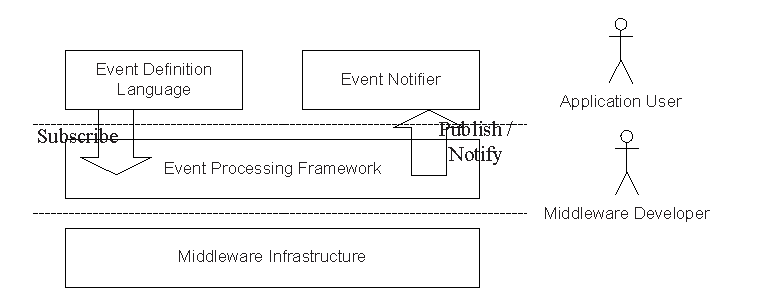
\includegraphics[width=\textwidth]{programmingModel}
\caption{PSWare programming model}
\label{fig:programmingModel}
\end{figure}

As shown in Figure \ref{fig:programmingModel}, our model mainly has two different types of people that make use of two APIs of different levels:
\begin{itemize}
\item Application developers make use of the PSWare-EDL to define and subscribe events and use the event receiving module to receive the published events.
\item Middleware developers make use of the event processing framework to implement effective and efficient event processing algorithms. The event processing framework may be further divided into two layers for event detection and event delivery.
\end{itemize}

The first type is the application users. These users are responsible for defining and subscribing to high level events for different types of applications. They use a high level event definition language (PSWare-EDL) to translate the application requirements into events. They do not have to worry about the underlying event processing mechanisms.

On the lower level, we have another type of users called middleware developers. These users are responsible for implementing domain-specific event processing mechanisms. PSWare provides a couple of interfaces in TinyOS to make the implementation easier.

The benefit for such a model lies in its flexibility. There are usually many different types of applications for a specific application domain. For example, in ITS, we may have collision warning, traffic flow control and overspeed detection yet these applications can probably share a lot of common event processing mechanisms. Therefore, the middleware developer only needs to implement the event processing mechanism for once. Then, by defining different events, we can easily meet different application requirements without sacrificing the efficiency.

\subsection{PSW-EDL: Event Definition Language in PSWare}
\begin{figure}
\centering
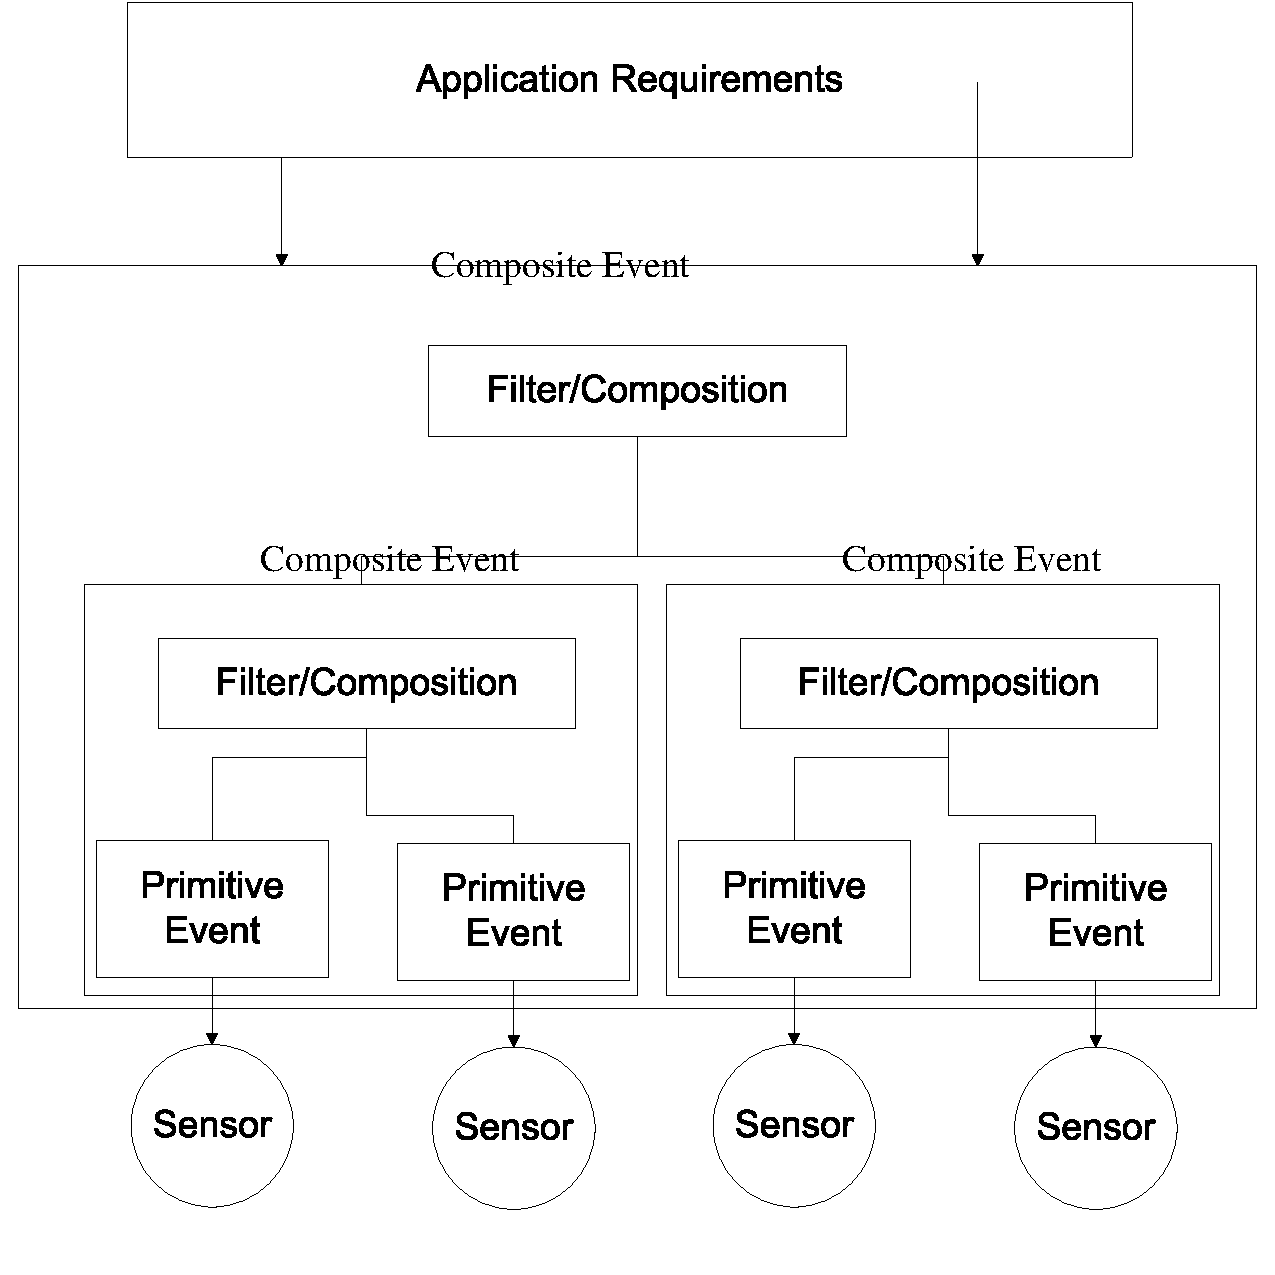
\includegraphics[width=.6\textwidth]{eventprogramming}
\caption{Type-based event model}
\label{fig:eventprogramming}
\end{figure}

PSWare provides a type-based event programming model to the application user. Such model has the following characteristics:
\begin{itemize}
\item Each event type is similar to a class in object-based programming model. Similarly, event hierarchy in Figure \ref{fig:eventhierarchy} is similar to class hierarchy.
\item Similar to object-based model, attributes are encapsulated in each event.
\item Event definition is declarative. The high-level application developers only need to specify the event filters and event relations through operators and functions. The underlying mechanisms for implementing these operators are left to our event processing framework.
\end{itemize}

Figure \ref{fig:eventprogramming} conceptually shows our event model. On the top level, the application requirements are expressed in terms of the composite events that need to be detected. The composite events may be further divided into sub-events. Eventually all composite events can be divided into primitive events which can be directly detected by individual sensor nodes.

\begin{figure}
\centering
\subfloat[Centralized]{\label{fig:room-a}\figurehalfwidth{room-a}}
\subfloat[Distributed]{\label{fig:room-b}\figurehalfwidth{room-b}}
\caption{Motivating application for indoor monitoring}
\label{fig:rooms}
\end{figure}

To illustrate using an example, consider a monitoring application shown in Figure \ref{fig:rooms}. The composite event consists of two sub-events to be detected in two different rooms, Room A and Room B. It occurs when the temperature in room A rises to a certain threshold and after 5 minutes, the temperature in room B also reaches that threshold. We may define the events as shown in Listing \ref{lst:rooms}.
\begin{lstlisting}[caption=Example of using event-based programming model, float, label=lst:rooms]
Event SimpleEvent {
	int temp=System.temp;
	int id=System.id;
	int time=System.time;
} where {
	temp > 30
}
Event CompEvent {
} on {
	SimpleEvent e1 and
	SimpleEvent e2
} where {
	e1.Location="A" and
	e2.Location="B" and
	e2.time-e1.time=600
}
\end{lstlisting}

We can see that our event-based programming model shares some of the similarity with SQL, especially for the event filters, which consist of operators. In this particular example, we have two event types. On the top level, the application wants to monitor the temperature change so the event type 'CompEvent' is defined. 'CompEvent' consists of two sub-events of the same type: SimpleEvent. Note that our programming model is declarative. The user just specifies the event types and the corresponding filters without specifying the event processing methods because that part is left to the event processing framework. We will go into more details in that in the latter part of this section.

\subsection{PSW-EN: Event Notifier in PSWare}
Apart from submitting event definition, the application user needs to be notified when the subscribed events are detected by WSN. This is done through event notifier. When the application user subscribes events, the user needs to pass an additional object as the event notifier. When the subscribed event is detected, PSWare will notify the user with this notifier object. Listing \ref{lst:notiferJava} shows our notifier class implemented and how it is related to the subscription class.

\begin{lstlisting}[caption=Event notifier in Java, label=lst:notiferJava]
public interface EventNotifier {
	public void notify(String eventStr);
	...
}
public class EventSubscription {
	public Boolean subscribe(String subscription, EventNotifier notifier) {
		...
	}
}
\end{lstlisting}

While Listing \ref{lst:notiferJava} shows the notifier in Java, bindings for other languages can be created in similar fashion. A Python binding is shown in Listing \ref{lst:notiferPython}.
\begin{lstlisting}[caption=Python binding of event notifier, label=lst:notiferPython]
class EventNotifier:
	def notify(self, eventStr):
		pass
class EventSubscription:
	def subscribe(self, subscription, notifier):
		...
\end{lstlisting}

Upon the detection of events, the notifier will be invoked so that the events can be delivered to the user. The event is delivered as a string, with each attribute assigned with an actual value. As an example, suppose the user has subscribed to the event 'SimpleEvent' in Listing \ref{lst:rooms}, then when the event is detected by PSWare, it will be delivered to the user with the content shown in Listing \ref{lst:eventFormat}.
\begin{lstlisting}[caption=Received event from notifier, label=lst:eventFormat]
SimpleEvent e1 {
	temp=32;
	id=0;
	time=13345;
}
\end{lstlisting}

\subsection{API for Event Processing Framework}
The event processing framework of PSWare is developed using NesC. PSWare also provides a group of APIs for the middleware developers to write customized event processing mechanisms. First, since all events can ultimately be decomposed into primitive events, the middleware developer needs to first define the required primitive events used in the application domain. This is done through a configuration named 'PrimitiveEventC'. It is listed in Listing \ref{lst:primitiveEvent}. The new event ID should be defined as an enumeration in PSWare's header file.
\begin{lstlisting}[caption=Primitive event component in NesC, label=lst:primitiveEvent]
generic configuration PrimitiveEventC(evet_id_t eventId) {
  provides {
    interface Read<uint16_t>;
  }
} implementation {
	...
}
\end{lstlisting}

In PSWare, everything is treated as an event and that includes temperature, photo and even timer. Similar to other generic components in TinyOS, if necessary, new events can be added by defining a new event ID. Once set, we need to create a higher level primitive event so that the application users can make new event definitions based on top of it. This is done by an automatic tool which will be invoked when building and output a class which will be used by the event notifier and an event definition which will be used by EDL.

When this is set, the application user can already start to subscribe and detect events by using PSWare's default event detection algorithm: TED \cite{lai:ted}. If the middleware developer wants to write their own event detection algorithm, they can choose to implement two interface 'EventMatcher' and 'EventDeliver' as shown in Listing \ref{lst:pswareEventMatcher}. The 'EventMatcher' interface includes two major events which serve three purposes as follows:
\begin{enumerate}
\item During the execution of the middleware, the network may detect multiple events for a single event type. Therefore, upon the detection of the composite events, the event detection algorithm may choose a specific event from one of this sub-types for detection. This is done by signaling the first event 'select sub-event'.
\item Upon the detection of an event, the event detection algorithm may perform some customized processing to update some information so that the next time when the event happens again, it may be detected with lower cost. This is when the second event 'eventMatched' comes into play. The middleware developer may implement customized event processing mechanisms according to the matched events.
\end{enumerate}

Apart from event matcher, we also have an event deliverer which will be invoked when a subscribed event is detected. The middleware developer may implement its only function to meet the requirements for event delivery. This is done when the middleware signals the 'eventDeliver' event.
\begin{lstlisting}[caption=The event matcher interface, label=lst:pswareEventMatcher]
interface EventMatcher {
	event bool selectSubevent(EventInstanceInfo * composite, EventInstanceInfo * subevent);
	event result_t eventMatched(evet_id_t eventId, evet_id_t instanceID, bool detectionResult);
}
interface EventDeliverer {
	event result_t eventDeliver(evet_id_t eventId, evet_id_t instanceID, bool detectionResult);
}
\end{lstlisting}

To facilitate the implementation of event matcher and event deliverer the middleware developer can make use of the APIs provided by PSWare in Listing \ref{lst:pswareAPI}. These APIs are mostly used to retrieve the event information.

The first interface, 'EventType' has four commands. The first command is for the individual event instances to obtain the type information based on their type ID as shown on line \ref{lst:pswareAPI:typeID}. The second and the third commands are used to determine if a given event type is a composite event or is subscribed by the user. The last command is for query the relation of e2 in reference to e1. Its return type is an enumerate which can have value of: parent, immediate parent, child and immediate child. This command will be useful if the user wants to implement customized event processing mechanisms.

\begin{lstlisting}[caption=PSWare API in NesC, float, label=lst:pswareAPI]
interface EventType {
	command EventTypeInfo * getEventType(evet_id_t eventId);
	command bool isSubscribed(evet_id_t eventId);
	command bool isComposite(evet_id_t eventId);
	command EventRelation getRelation(event_id_t e1, event_id_t e2);
}
interface EventInstance {
	command int instanceAmount(evet_id_t eventId);
	command EventInstanceInfo * getEventInstance(evet_id_t eventId, evet_id_t idx);
	command void deleteEvent(evet_id_t eventId, evet_id_t instanceID);
}

typedef struct {
	evet_id_t eventId;
	evet_id_t level;
	size_t size;
} EventTypeInfo;

typedef struct {
	evet_id_t typeID; (*\label{lst:pswareAPI:typeID}*)
	evet_id_t instanceID;
	uint16_t * attributes;
} EventInstanceInfo;
\end{lstlisting}

Since for each event type, there can be multiple events, we need the second interface 'EventInstance' to process those events. There are three commands for this interface. The first one is used to obtain the number of the events for a specific type currently stored in the event buffer on the sensor node. We will discuss about the event buffer in the next section. Upon knowing the number of events, the middleware developer can iterate through the event list and use the second command to get the events. As for the last command, when an event is detected to be useless, the middleware developer may delete it from the list.

The data structures are shown after the interfaces. For a given event type, we have the ID for the type, its level in the subscribed event tree and its size. For the event instance data structure, we have its type ID, instance ID and its attribute list. If the event contains some attributes of the primitive events, they can be obtained here by using the index defined in the enumeration value for primitive event. For instance, if one of the primitive event has an enumeration value labeled 'EVENT\_LIGHT', then if the event instance also has one of its attribute from the sensor's light reading, the middleware developer can access it by writing 'attributes[EVENT\_LIGHT]'.

In summary, the middleware developer may follow the following steps to implement customized event processing mechanisms:
\begin{itemize} 
\item Implement new primitive event types if necessary.
\item Define the event matcher for how sub-events are selected for matching and what to do after a predefined event type is detected.
\item Define customized function for event delivery.
\end{itemize}